\documentclass[a4paper,10pt]{scrartcl}
\usepackage[utf8]{inputenc}
\usepackage{graphicx}

%opening
\title{Quadcopter Project Proposal}
\subtitle{ROBO 410 Dr. Mark Yoder}
\author{Team Bone and Team Sky: \\
	{\normalsize Bryce Filho (filhobc@rose-hulman.edu) }\\
	{\normalsize Chris Hopwood (hopwoocp@rose-hulman.edu) }\\
	{\normalsize Michael McDonald (mcdonamp@rose-hulman.edu) }\\
	{\normalsize Shawn Mitchell (mitchesm@rose-hulman.edu) }\\
	{\normalsize Daniel Nam (namdw@rose-hulman.edu) }\\
	{\normalsize Ryan Oliver (oliverr@rose-hulman.edu) }\\
	{\normalsize Justin Stone (stonejp@rose-hulman.edu) }\\
	{\normalsize Elias White (whiteer@rose-hulman.edu) }\\
	}

\begin{document}

\maketitle

\newpage

\tableofcontents

\begin{table}[b]
\centering
\begin{tabular}{| l | l | p{7.5cm} |}
\hline
\textbf{Revision} & \textbf{Date} & \textbf{Comments}\\
\hline
1.0 & 9/25/2013 & Initial Copy \\
\hline
\end{tabular}
\end{table}

\newpage

\section{Executive Summary}
\noindent The goal of this project is to create a plug-and-play quadcopter
add-on, or cape, solution for the BeagleBone Black.  With the recent explosion
of quadcopters among hobbyists and researchers, a platform that is affordable,
powerful without being overwhelming, and expandable fills a unique niche in the
current market. With the release of TI's BeagleBone Black, a very capable yet
affordable embedded processor, all three of these goals are attainable. The
successful completion of this project would result in a mechanical design for
the quadcopter frame, a BeagleBone Cape that houses sensors and motor
controllers, integrated flight control software for in-flight stabilization, and
the ability to communicate with a control base. We will be leveraging both our
resources at TI as well as the open source community throughout the course of
our project, and plan on open sourcing the mechanical designs, PCB schematic and
layout files, and source code.

\newpage
\section{Walkthrough}
\noindent The client contact at TI (currently Jason Kridner, the main software
developer on the Beagle Board/Bone platform) wants a quadcopter expansion
board/cape for the BeagleBone Black that is out of the box ready to fly or
almost ready to fly quadcopter, yet can still be expanded upon by the
hobbyist community and the users themselves. \\

\noindent The QuadCape and BeagleBone Black can be ordered on the client’s
website or through selected third party distributors. Upon delivery, the
customer will open the packaging and assemble the kit by attaching the
BeagleBone Black to the QuadCape, and attaching motors, propellers, and a
battery (all of which are either shipped with the kit or provided by the
user). \\

\noindent After enabling flight mode by pressing the on switch on the cape, an
LED will light indicating that the quadcopter has power and it's sensors have
been initialized. The quadcopter will then begin to fly; stably and slowly
raising altitude relative to its initial altitude. The user will then be able to
control the quadcopter via wireless communication: either a laptop or a mobile
device (phone or tablet). \\

\noindent To add functionality to the quadcopter, the customer can add software
through the continually evolving open source community that already exists
around the BeagleBone. The customer can also add hardware to the quadcopter
through any of the multiple ports of the BeagleBone Black by adding capes or
modifying the QuadCape board and building one themselves. If the user happens to
break anything, parts for the QuadCape or the quadcopter frame will be available
for purchase, and the design files will be published so users could build their
own replacements. Through this open source community the quadcopter will have
greater opportunity to be any type of project the client chooses, and will boost
the reputation of TI and the BeagleBone.

\newpage
\section{Domain Model}
\begin{figure}[h]
 \centering
 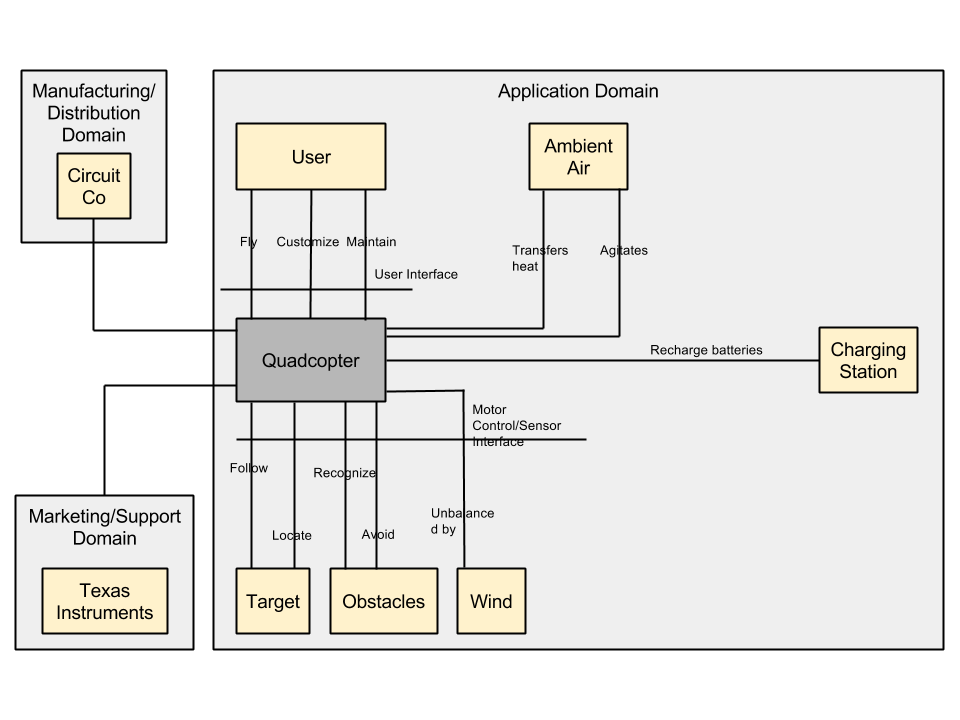
\includegraphics[scale=0.5]{./DomainModel.png}
 % Domain Model.png: 960x720 pixel, 72dpi, 33.87x25.40 cm, bb=0 0 960 720
 \caption{Domain Model}
\end{figure}

\newpage
\section{Stakeholder Model}
\begin{center}
\begin{tabular}{| l | p{7.5cm} |}
\hline
\textbf{Stakeholder} & \textbf{Features}\\
\hline
Dr. Mark Yoder and Rose-Hulman & \emph{Documentation}: should be reproducible,
allow for easy future use and modification\newline
\emph{Manufacturing Cost and Time}: should be a completed product within spec
and budget, maintain/improve relationship with Texas Instruments\newline
\emph{Safety}: should be safe to build/test, as well as operate in the
future\newline
\emph{Operation Costs}: should not require special equipment or additional
overhead to use in the future\\
\hline
Jason Kridner and Texas Instruments & \emph{Customization}: should allow for
user customization, act as a marketing tool to sell additional TI products
\emph{Documentation}: should be reproducible, portable to other TI
controllers/launchpads\newline
\emph{Manufacturing Cost and Time}: should be cheap and quick to manufacture in
order to sell at a reasonable price and be more appealing than building a
quadcopter from scratch\\
\hline
CircuitCo & \emph{Customization}: should allow for expansion, without
interfering with original design and manufacturing process, may provide other
manufacturing/sales opportunities\newline
\emph{Durability}: should be well-designed and not require replacements under
warranty for normal usage\newline
\emph{Manufacturing Cost and Time}: should be efficient to manufacture, minimal
waste\newline
\emph{Maintenance}: should not require extensive hardware support\newline
\emph{Packaging}: should fit into a standard package and minimize inventory
space, be easy to ship individually and in bulk\newline
\emph{Regulatory Compliance}: should be designed to meet regulations and not
interfere with or delay the manufacturing process\\
\hline
\end{tabular}
\end{center}

\newpage
\begin{center}
\begin{tabular}{| l | p{7.5cm} |}
\hline
Hobbyist Community & \emph{Customization}: should act as a platform for design
and experimentation, should be easy to incorporate other projects, remain
open source\newline
\emph{Durability}: should be able to withstand testing and experimentation,
avoid severely damaging components\newline
\emph{Maintenance}: should be supported into its life cycle, offer replacement
parts or firmware updates\newline
\emph{Safety}: should not be a hazard to the operator or bystanders, or be
unnecessarily dangerous to modify\newline
\emph{Reliability}: both hardware and software should be robust, as countless
hours and funds may be invested into projects revolving around the
product\newline
\emph{Ease of Use}: should be easy to operate and interface with, more appealing
than building a quadcopter from scratch\newline
\emph{Operation Costs}: should not require special equipment or additional
overhead to use in the future\\
\hline
Educational Community & \emph{Customization}: should act as a platform for
design and experimentation, should be easy to incorporate other projects, remain
open source\newline
\emph{Durability}: should be able to withstand testing and experimentation,
avoid severely damaging components, resistant to student misuse
\emph{Maintenance}: should be supported into its life cycle, offer replacement
parts or firmware updates, should require minimal technical knowledge to keep
product operational\newline
\emph{Safety}: should not be a hazard to the operator or bystanders, or be
unnecessarily dangerous to modify, should be safe to use around
children/students\newline
\emph{Reliability}: both hardware and software should be robust, as countless
hours and funds may be invested into projects revolving around the
product\newline
\emph{Ease of Use}: should be easy to operate and interface with, more appealing
than building a quadcopter from scratch, should require minimal technical
knowledge to operate the completed product\newline
\emph{Operation Costs}: should not require special equipment or additional
overhead to use in the future\\
\hline
Regional Community & \emph{Environment Friendly}: should not harm the
environment through operation, provide options for disposal or recycling\newline
\emph{Safety}: should be safe to operate within a community, on a larger scale\\
\hline
\end{tabular}
\end{center}


\newpage
\section{State Model}
\begin{figure}[h]
 \centering
 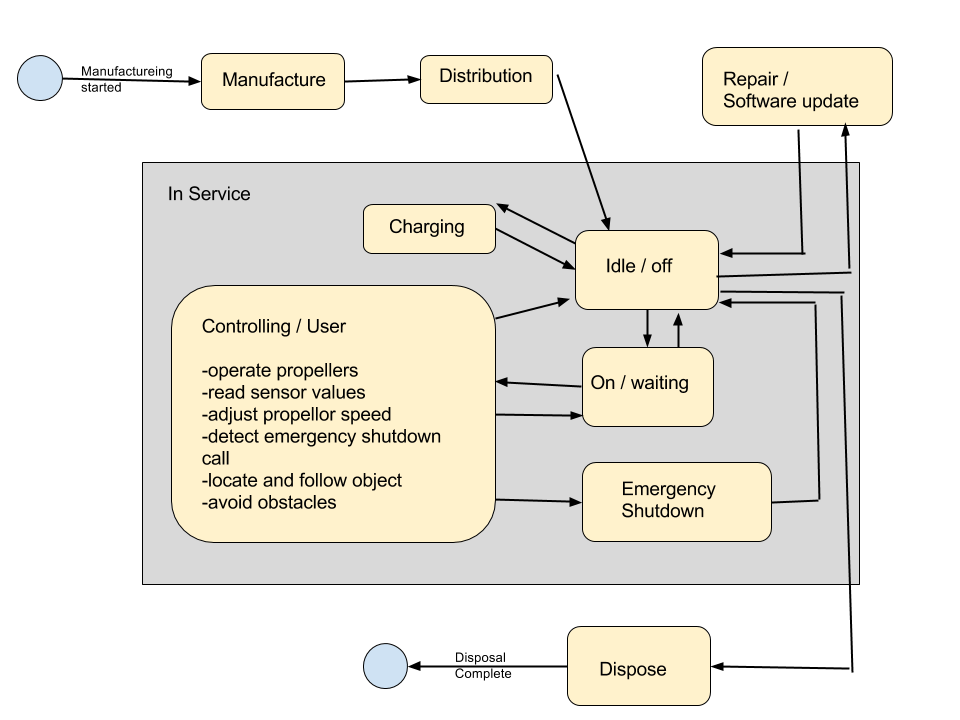
\includegraphics[scale=0.5]{./StateDiagram.png}
 % State Diagram.png: 960x720 pixel, 72dpi, 33.87x25.40 cm, bb=0 0 960 720
 \caption{State Diagram}
\end{figure}


\newpage
\section{Logical Architecture}
\begin{figure}[h]
 \centering
 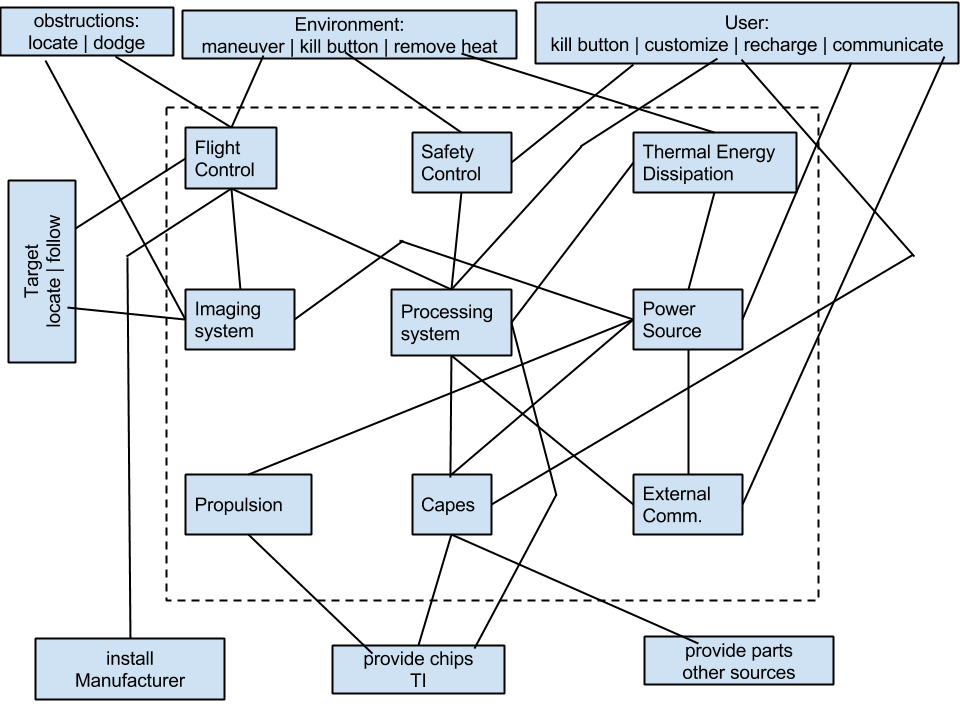
\includegraphics[scale=0.5]{./Logicblockdiagram.png}
 % Logic block diagram.png: 960x720 pixel, 72dpi, 33.87x25.40 cm, bb=0 0 960 720
 \caption{Logical Architecture}
\end{figure}


\end{document}
